\chapter*{Введение}							% Заголовок
\addcontentsline{toc}{chapter}{Введение}	% Добавляем его в оглавление

В настоящее время все более популярным и распространенным становится процесс передачи функций поддержки информационной инфраструктуры (далее~--- ИТ-инфраструктуры) предприятия какой-либо внешней компании (см., например, \cite{StartToOutsource}). Это явление стало называться «ИТ-аутсорсинг» (от анг. ”out source”~--– вне источника). С развитием рынка информационных систем компаниям становится невыгодно держать свой штат службы поддержки, и они отдают эти функции сторонней компании (см. \cite{OutsourceEff}). В некоторых случаях передаются все функции поддержки пользователей: будь-то заявка на ремонт компьютера или же информационный запрос, возникающий из-за простого незнания внутренних процессов компании. В результате создается единая точка входа для пользователей, поддерживаемая сторонней компанией \cite{OutsourceSD}. Обобщая, можно сказать, что на аутсорсинг передают все, что возможно: управление персоналом, уборку помещений, обеспечение питанием, разработку программного обеспечения (далее~--- ПО) (см., например, \cite{OutsourceSoft}) \etc \par
В некоторых областях, например, в области информационных технологий (ИТ) за счет аутсорсинга экономия средств предприятия достигает 30\% (по данным Gartner \cite{OutsourceIT}).
Из-за возросшей популярности бизнеса по аутсорсингу именно в ИТ-области и появления большого количества компаний возникла сильная конкуренция \cite{AUTOS-1}, что привело к снижению цен на услуги и потребовало сокращения издержек компаний. Для поиска путей оптимизации издержек было необходимо применение методов системного анализа для решения сложившихся проблем \cite{AUTOM-1}. Также было отмечено падение рентабельности бизнеса как минимум для малых компаний \cite{OUTSOURCE-RENT}, \cite{OutsourceEff}. В контексте оптимизации издержек в настоящей диссертации рассматриваются модель области, модель системы и ее реализация, которая повышает эффективность работы специалиста технической поддержки (далее специалист) путем частичной (в некоторых случаях, полной) автоматизации обработки инцидентов (случаев, происшествий)  \cite{SDAUTOM}, начиная с разбора запросов, сформулированных на естественном языке, и заканчивая применением найденного решения. \par
Главным требованием к системе повышения эффективности ИТ-службы предприятия является замена части функций, которые сейчас выполняют специалисты:
\begin{enumerate}
  \item Обработка запросов на естественном языке~--- эта функция широко востребована и в системах анализа проблем пользователя с построением статистики «Удовлетворенность пользователя программным продуктом» \cite{TUTUB-1}. Общее понимание проблемы зависит от понимания языка, на котором общаются специалисты;
  \item Возможность обучения. Такая возможность системы позволяет упростить ее эксплуатацию и расширение. По данным исследования \cite{LEARN-1}, возможность обучения очень важна для любой интеллектуальной системы, включая системы управления роботами. Обучение обеспечивает системе большие гибкость и универсальность;
  \item Общение со специалистом. Поддержание диалога (коммуникации)~--- необходимое условие для обучения. Кроме того, социальная функция~--- неотъемлемая часть интеллектуальных систем (см., например, \cite{LEARN-2});
  \item Проведение логических рассуждений (возможность размышлять): аналогия, дедукция, индукция~--- умение обобщить решение одной проблемы и, экстраполируя его, применить для решения других. Иными словами, это возможность для системы принять правильное решение. Например, принятие решений широко используется в интеллектуальных системах управления производством  \cite{LEARN-3}.
\end{enumerate}

На данный момент времени многие компании ведут в различных областях разработку подобных систем, обладающих свойствами, описанными выше. Системы такого класса также называются \textit{вопросно-ответными}. Примером является набирающая популярность IBM Watson \cite{WATSON-PO}, \cite{WATSON-PTOP} (которая является коммерческой и закрытой, информации о ее внутреннем устройстве мало). Другой пример~--- компания HP использует результаты исследования \cite{TUTUB-2} для автоматического определения проблем и степени удовлетворенности пользователей из отчетов об использовании программного обеспечения. Также эта компания работает над автоматическим решением проблем (как описано выше). \par

В настоящей диссертации представлены результаты и апробации создания вопросно-ответной системы на основе исследования целевой области (удаленная поддержка информационной инфраструктуры предприятия) и построения модели системы. Акцент был сделан на создании интеллектуальной системы для решения широкого круга проблем. \par

Следует отметить, что большинство проблем, которые решает удаленная служба поддержки информационной инфраструктуры предприятия, носит достаточно тривиальный характер (по данным компании \icl): установить приложение; переустановить приложение; решить проблему с доступом к тому или иному ресурсу.
Названные проблемы решают специалисты технической поддержки, которая обычно делится на несколько линий по уровню умения специалистов. Каждая линия поддержки представлена своим классом специалистов. В среднем команда, обслуживающая одного заказчика, насчитывает около 60 человек. Процентное соотношение специалистов разных линий поддержки отображено на рисунке \ref{img:ITSMTeamComposition}.

\begin{table} [htbp]
  \centering
  \parbox{15cm}{\caption{Описание работы специалистов различных уровней поддержки}\label{TSSDescription}}
%  \begin{center}
  \begin{tabular}{| p{7cm} | p{7cm} |}
    \hline
\textbf{Уровень} & \textbf{Описание} \\
  \hline
    

Первая линия	& Решение уже известных, задокументированных проблем, работа напрямую с пользователем \\
  \hline

Вторая линия  & Решение ранее неизвестных проблем \\
  \hline

Третья линия & Решение сложных и нетривиальных проблем \\
  \hline

Четвертая линия  & Решение архитектурных проблем инфраструктуры \\

  \hline
  
  \end{tabular}
%  \end{center}
\end{table}



\begin{figure} [h] 
  \center
  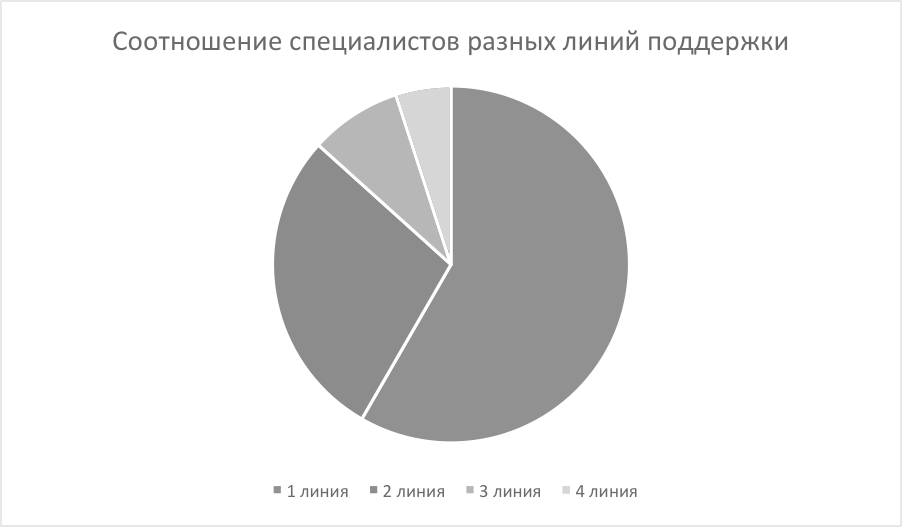
\includegraphics [scale=0.7] {ITSMTeamComposition}
  \caption{Диаграмма состава команд} 
  \label{img:ITSMTeamComposition}  
\end{figure}

Работа специалистов первой линии поддержки состоит из множества рутинных и простых задач. На рисунке \ref{img:EngineerTasks} показано соотношение разных типов проблем, встречающихся во время работы службы поддержки, в таблице \ref{IncidentDescription} приведена расшифровка типов. Данные подготовлены на основе анализа работы команд \icl.

\begin{figure} [h] 
  \center
  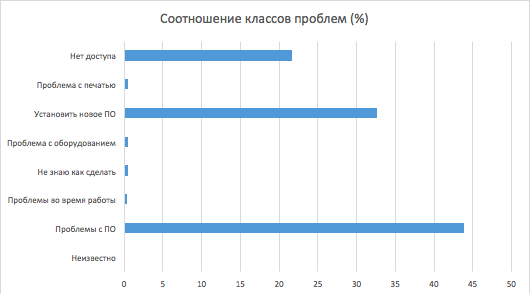
\includegraphics [scale=0.7] {EngineerTasks}
  \caption{Диаграмма соотношений типов проблем} 
  \label{img:EngineerTasks}  
\end{figure}

\begin{table} [htbp]
  \centering
  \parbox{15cm}{\caption{Категории инцидентов в области удаленной поддержки инфраструктуры}\label{IncidentDescription}}
%  \begin{center}
  \begin{tabular}{| p{7cm} | p{7cm} |}
 
  \hline
\textbf{Категория} & \textbf{Описание} \\
  \hline
Проблема с ПО	& Проблема при запуске ПО на компьютере. Решается переустановкой \\
  \hline
Проблемы во время работы  & Проблема с функционированием программного обеспечения\\
    \hline
Как сделать & Запрос на инструкцию по работе с тем или иным компонентом рабочей станции \\
      \hline
Проблема с оборудованием  & Неполадки на уровне оборудования \\
  \hline
Установить новое ПО       & Требование установки нового программного обеспечения \\
  \hline
Проблема с печатью        & Установка принтера в систему \\
    \hline
Нет доступа               & Нет доступа к общим ресурсам \\
  \hline
  \end{tabular}
%  \end{center}
\end{table}

Как показывают исследования, решение части задач может быть автоматизировано. Если это будет сделано,  специалисты получат дополнительное время для решения более сложных задач. \par
\textbf{Применение моделей теории массового обслуживания}.
Рассмотрим модель данной системы в разрезе теории массового обслуживания (ТМО). Она может быть выражена в виде входящего потока заявок (инцидентов), очереди и нескольких агентов (специалистов, автоматизированных систем). 
Важно отметить, что на время обработки заявки агент блокируется и не может принимать новые заявки. На Рисунке \ref{img:mass_service} представлена модель системы массового обслуживания в ИТ. 
  
\begin{figure} [h] 
  \center
  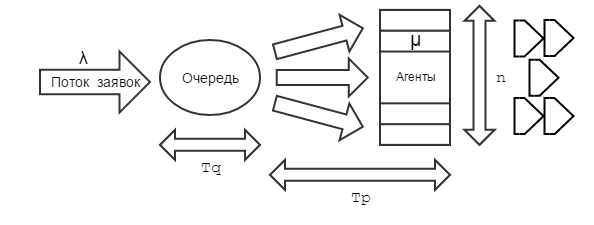
\includegraphics [scale=0.8] {mass_service}
  \caption{Модель системы массового обслуживания в ИТ.} 
  \label{img:mass_service}  
\end{figure}

Здесь \ref{img:mass_service} $\lambda$ --- интенсивность входящего потока;
$\alpha$ --- доля заявок, для которых время в очереди превышает $T_qmax$;       
$\mu$ --- величина, обратная среднему времени нахождения заявки у агента;
n --- число агентов;
$T_q$ --- время нахождение заявки в очереди в часах;
$T_qmax$ --- максимально допустимое время ожидания;
SLA --- уровень обслуживания (1-$\alpha$), доля заявок, для которых время в очереди не превышает $T_qmax$. $T_p$ --- время удовлетворения заявки;
 $\alpha_n$ --- количество заявок;
 $T_{qp}=T_q+T_p$ --- время прохождения заявки через систему;
 $S(\mu)= \frac{R_p}{\mu} $ --- средняя стоимость выполнения одной заявки;
 $R_p$ --- средняя стоимость часа работы специалиста (выводится далее).
 \par
Существует несколько методов решения задачи ТМО: 
\begin{itemize}
	\item Аналитическое решение для простейших систем, которое позволяет выразить $T_q (t)$ через $\lambda$, $\mu$ и n;
	\item Для более сложных систем, где вводятся дополнительные параметры: приоритеты заявок, 
	последовательная эскалация инцидентов \etc, строится гистограмма $T_q (t)$, по которой оценивается достаточность n для обеспечения SLA (имитационный подход);
	\item Для систем с достаточно большим n возможно оценить $T_q (t)$ по имеющейся статистике (эконометрический подход).
\end{itemize} \par
В \cite{TMO} на основе комбинации формулы Эрланга, модели Энгсета и модели Полячека~-~Хинчина 
построена формула для решения аналитической задачи нахождения распределения вероятностей для $T_qp$. Основной же задачей этой работы является прогнозирование необходимых ресурсов для $max SLA$. 
В данной диссертации ставится задача $min T_{qp}$, $min S(\mu)$ и динамического выделения ресурсов. На основе  статистики, собранной в компании \icl~ был подсчитан следующий коэффициент $T_{qp}=47,9$ при $n=6$; $SLA=0,82$; $\alpha=0,18$;  $\alpha_n=2920$. 
Для анализа потока заявок в данном случае лучше использовать имитационный подход, так как n слишком мало. На Рисунке \ref{img:LAMBDAAV} представлен средний поток заявок по часам, посчитанный на основе собранной статистики. На нем наглядно видно как меняется поток с течением дня.

\begin{figure} [h] 
  \center
  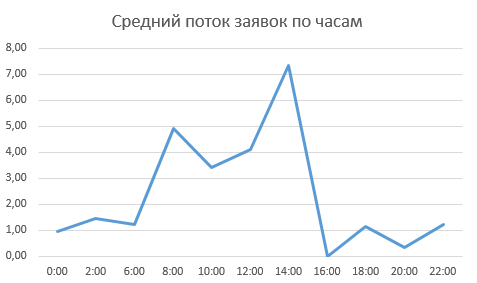
\includegraphics [scale=1.0] {LAMBDAAV}
  \caption{Средний поток заявок по часам.} 
  \label{img:LAMBDAAV}  
\end{figure}



\textbf{Предпосылки развития в изучаемой предметной области}. 
Основной тенденцией в развитии области удаленной поддержки ИТ-инфраструктуры являются попытки удешевить и улучшить стоимость предоставления услуг \cite{OutsourceEff}. \par
Компании, работающие на этом рынке, вкладывают большие средства в автоматизацию. Кроме того, современное развитие науки и техники, точнее, вычислительных мощностей \cite{SuperComputer} позволяет провести автоматизацию даже самых наукоемких процессов. Дальнейшей перспективой развития области является замена человеческих специалистов автоматизированными системами. Разработки в этом направлении ведут многие компании, например, компания HP, которая имеет свою систему регистрации различных инцидентов \cite{HPOpenView} и сейчас ведет работу над ее автоматизацией. В качестве некоторого сравнения можно провести параллель происходящего процесса с промышленной революцией XVIII–XIX веков (см., например, \cite{IndustrialRev}). \par
\textbf{Обзор исследований в изучаемой предметной области}. 

Область исследования, с которой связана диссертация, является комплексной и включает в себя различные направления работ, в частности, создания различных интеллектуальных систем. Сфера применения интеллектуальных систем обширна, например, в Институте Чиная (Индия) Е. Джубилсоном и П. Дханавантини ведутся исследования интеллектуальных систем обработки запросов пользователей в области телекоммуникаций \cite{CHIN-1}, а в университете Ганновера (Германия) Р. Брунс и Дж. Данкель разрабатывают интеллектуальные системы для обработки запросов в службу спасения с целью уменьшения времени реакции на происшествие \cite{Dunkel}. В Санкт-Петербургском государственном университете под руководством В.И. Золотарева проводится оценка эффективности службы информационной поддержки в Вычислительном центре СПбГУ \cite{SPB}. В Сингапуре С. Фу и П. Леонг проведен анализ эффективности ИТ-службы поддержки крупной компании и показана возможность автоматизации ряда процессов \cite{SING}.\par
Исследования в области интеллектуальных систем повышения эффективности ИТ-службы предприятия ведутся также лидерами отрасли: компаниями HP \cite{HPOpenView} и IBM \cite{WATSON-PO}. Например, известна многоцелевая интеллектуальная система IBM Watson, разработкой и исследованием которой занимается группа под руководством профессора А. Гоэля (США--Китай).  \par   

Еще одно из направлений исследований в области обработки естественного языка составляет подход GATE \cite{GATE-1}, который активно развивается в университете Шеффилда (Великобритания) под руководством Г. Каллаган, Л. Моффат и С. Сзаз. Другое направление~--- это семантический поиск, исследования в этой области также активно ведутся в университете Шеффилда, в частности, выработан подход "Mimir"\,, который реализует возможности поиска по принципу «поиск и открытие» \cite{MIMIR}. Для организации поиска решений в соответствии с запросами пользователей в таких системах используются онтологии, например, широко применяется подход, предложенный С. Дей и А. Джеймс из Калифорнийского университета (США), основанный на применении деревьев тегов в онтологии \cite{ONTCON}. \par
Для придания интеллектуальной системе гибкости необходимо дать ей возможность проводить логические рассуждения. Одной из ведущих организаций в этом направлении исследований является консорциум OpenCog \cite{OpenCog} (США). Этими работами руководит Бен Герцель (председатель Artificial General Intelligence Society и OpenCog Foundation)~--- один из мировых лидеров в области искусственного интеллекта. Исследования в области машинной логики также ведутся в рамках проекта NARS \cite{NARS} под руководством профессора университета Темлпа (США) Пея Вонга. \par 

Интерес к области интеллектуальных систем обработки информации можно, в частности, оценить как количество публикаций за последние годы, процитированных в базе данных Scopus,~--- с 2004 года в среднем оно составило около 1010 в год. \par
\textbf{Стандарты, используемые в области ИТ-аутсорсинга: ITIL и ITSM} \par
В области ИТ-аутсорсинга есть несколько готовых стандартов ведения работ, одним из которых является библиотека ITIL. Этот стандарт описывает лучшие практики организации работ в области ИТ-аутсорсинга. Используемый в библиотеке подход соответствует стандартам ISO 9000 (ГОСТ Р ИСО 9000) \cite{ITIL1, ITIL2, ITIL3}.
Наличие стандартов диктует унифицированность как постановки проблем, так и алгоритмов решения, а также способствует возможности частичной или в некоторых случаях полной автоматизации решения проблем. \par
\clearpage
\textbf{Оценка стоимости работы специалиста} \par
По данным аналитики портала SuperJob \cite{SuperJob}, в Казани среняя зарплата системного администратора с опытом работы в 2014 году составляла 30 – 35 тыс. руб. (из расчета на 1 час с учетом 21 рабочего дня в месяце~--- 179--208 руб. в час). В соответствии с действующим российским законодательством \cite{FiscalCodecs} расходы компании на одного работника определяются по формуле
\[
L = R + R*(F_1 +F_2+F_3),
\]
где R~--- выплата человеку в час, F1~--- НДФЛ 13\%, F2~--- совокупность отчислений в ФБ (6\%), ПФР (14\%), ТФОМС (2\%), ФФОМС (1,1\%), ФСС (2,9\%), F3~--- налог на прибыль (20\%). Таким образом, расходы компании на сотрудника варьируются от 285 до 314 руб. в час, а за 8-ми часовой рабочий день – от 2280 до 2512 руб. Далее, аренда выделенного сервера (Xeon X3, 1.7 GHz, 8GB RAM, 256GB SSD) стоит 8 900 руб./мес. (см. \cite{TimeWeb}) (53 рубля за 1 час ($R_p=53$ с учетом 8-ми часового рабочего дня). Но сервер может работать 24 часа в сутки за исключением простоев на обслуживание, которые обычно составляют не более 5\% времени. \par Итого: сервер работает 478,8 часов в месяц. С этой точки зрения эксплуатация сервера будет стоить 18,5 руб. в час ($R_p=18,5$). Один сервер в своем быстродействии может заменить несколько специалистов при решении соответствующих задач. Чтобы решение было экономически эффективным, необходимо, чтобы оно сокращало расходы как минимум на 30\% (по данным \icl). \par Грубый подсчет на основе стоимости часа и пропорции показывает, что работа специалиста~--- это 6\% работы сервера (без учета работы сервера параллельно над несколькими задачами). Таким образом, уровень разрешения инцидентов системой в 50\% выполнит требования по прибыли примерно на 186\%.

\clearpage
\textbf{Общая характеристика диссертации} 
\newcommand{\actuality}{\underline{\textbf{Актуальность темы.}}}
\newcommand{\aim}{{\textbf{Целью}}}
\newcommand{\tasks}{{\textbf{задачи}}}
\newcommand{\scope}{{\textbf{Область исследования}}}
\newcommand{\subject}{{\textbf{Предметом исследования}}}
\newcommand{\methods}{{\textbf{Методы исследования}}}
\newcommand{\defpositions}{{\textbf{Основные положения, выносимые на~защиту:}}}
\newcommand{\novelty}{{\textbf{Научная новизна}}}
\newcommand{\influence}{{\textbf{Практическая значимость.}}}
\newcommand{\reliability}{{\textbf{Достоверность}}}
\newcommand{\probation}{{\textbf{Апробация работы.}}}
\newcommand{\contribution}{{\textbf{Личный вклад.}}}
\newcommand{\publications}{{\textbf{Публикации.}}}


{\aim} работы является разработка интеллектуальной системы повышения эффективности деятельности ИТ-службы предприятия. \par
{\scope}~--- разработка методов и алгоритмов решения задач системного анализа, оптимизации, управления, принятия решений и обработки информации в ИТ-отрасли.\par
{\subject}  является процесс регистрации и устранения проблемных ситуаций, возникающих в ИТ-инфраструктуре предприятия.\par

Для достижения поставленной цели необходимо было решить следующие {\tasks}:
\begin{enumerate}
  \item Провести теоретико-множественный и теоретико-информационный анализ сложных систем в области поддержки информационной инфраструктуры;
  \item Создать модель целевой области;
  \item Исследовать модели мышления и выбрать наиболее подходящую;
  \item На основе выбранной модели мышления разработать модель проблемно-ориентированной системы управления, принятия решений и оптимизации процесса принятия, анализа и обработки запросов пользователя в области обслуживания информационной структуры предприятия;
  \item Создать архитектуру приложения на основе модели;
  \item Реализовать на основе этой архитектуры прототип интеллектуальной вопросно-ответной системы повышения эффективности деятельности ИТ-службы предприятия;
  \item Провести апробацию прототипа на тестовых данных.
\end{enumerate}

\defpositions
\begin{enumerate}
  \item Теоретико-множественный и теоретико-информационный анализ сложных систем в области поддержки информационной инфраструктуры;
  \item Построенная модель проблемно-ориентированной системы управления, принятия решений и оптимизации технических объектов в области обслуживания информационной инфраструктуры;
  \item Созданный прототип программной реализации модели проблемно-ориентированной системы управления, принятия решений и оптимизации обработки запросов пользователя в области обслуживания информационной инфраструктуры;
  \item Апробация прототипа проблемно-ориентированной системы управления, принятия решений и оптимизации деятельности на контрольных примерах и анализ ее результатов.
\end{enumerate}

\novelty проведенного исследования состоит в следующем:
\begin{enumerate}
  \item Создана модель проблемно-ориентированной системы управления, принятия решений в области обслуживания информационной структуры предприятия на основе модели мышления;
  \item Представлены новая модель данных для модели мышления и оригинальный способ хранения для этой модели, эффективный по сравнению с другими базами данных;
  \item Выполнено оригинальное исследование моделей мышления применительно к области обслуживания информационной структуры предприятия;
  \item На основе модели мышления Мински созданы архитектура системы обслуживания информационной структуры предприятия и программный прототип этой системы.
\end{enumerate}

\influence\ 
Система, разработанная в рамках данной диссертации носит значимый практический характер. Идея работы зародилась под влиянием производственных проблем в ИТ-отрасли, с которыми автор сталкивался каждый день в процессе разрешения различных инцидентов, возникающих в деятельности службы технической поддержки \icl~--- одном из крупнейших системообразующих предприятий ИТ-области Республике Татарстан. Поэтому было необходимо выработать глубокое понимание конкретной предметной области, чтобы выбрать приемлемое решение, получившее практическое применение в работе на проекте поддержки крупной сети продуктовых магазинов. \par
\reliability\ научных исследований и практических рекомендаций
базируется на корректной постановке общих и частных рассматриваемых задач,  использовании известных фундаментальных теоретических положений системного анализа, достаточном объёме данных, использованных при статистическом моделировании, и широком экспериментальном материале, использованном для численных оценок достижимых качественных показателей. \par 
Исследования, проведенные в диссертации, соответствуют паспорту специальности 05.13.01~--- Системный анализ, управление и обработка информации, сопоставление приведено в таблице \ref{ResearchDescription}.

\begin{longtable}{|p{7cm}|p{9cm}|}
 \caption[Сопоставление направлений исследований в рамках специальности 05.13.01 и исследований, проведенных в диссертации]{Сопоставление направлений исследований в рамках специальности 05.13.01 и исследований, проведенных в диссертации}\label{ResearchDescription} \\ 
 \hline
 
 \multicolumn{1}{|c|}{\textbf{Направление исследования}} & \multicolumn{1}{c|}{\textbf{Результат работы}}  \\ \hline 
\endfirsthead
\multicolumn{2}{c}%
{{\bfseries \tablename\ \thetable{} -- продолжение}} \\
\hline \multicolumn{1}{|c|}{\textbf{Направление исследования}} &
\multicolumn{1}{c|}{\textbf{Результат работы}}  \\ \hline 
\endhead

\hline \multicolumn{2}{|r|}{{Продолжение следует}} \\ \hline
\endfoot

\hline \hline
\endlastfoot
\hline
   Разработка критериев и моделей описания и оценки эффективности решения задач системного анализа, оптимизации, управления, принятия решений и обработки информации & В рамках работы была разработана модель системы принятия решения и обработки информации в области решения запросов пользователя на естественном языке. \\
   \hline
   Разработка проблемно-ориентированных систем управления, принятия решений и оптимизации технических объектов & По модели, разработанной в предыдущем пункте был разработан прототип системы принятия решения Thinking Understanding, который был испытан на модельных данных.\\
   \hline
   Методы получения, анализа и обработки экспертной информации & В рамках системы TU был разработан метод обработки экспертной информации - обучение при помощи модели мышления TU, основанной на принципах модели 6-ти Марвина Мински. \\
   \hline
   Разработка специального математического и алгоритмического обеспечения систем анализа, оптимизации, управления, принятия решений и обработки информации & В рамках разработки системы TU были созданы специальные алгоритмы для анализа запросов пользователя и принятия решений.\\
  \hline 
  Теоретико-множественный и теоретико-информационный анализ сложных систем & В рамках работы был проведен комплексный анализ области поддержки программного обеспечения, с помощью которого была построена система данной области и выделены участки для оптимизации принятия решений.\\
  \hline
  Методы и алгоритмы интеллектуальной поддержки при принятии управленческих решений в технических системах & Система, разработанная в рамках данной работы в включает в себя инновационные методы и алгоритмы поддержки принятия решений, использующих в своей основе модель мышления на базе модели мышления Человека, описанной в книге Марвина Мински. \\ 
  \hline
  Визуализация, трансформация и анализ информации на основе компьютерных методов обработки информации & Представлена наглядная визуализация данных по системному анализу области удаленной поддержки инфраструктуры. \\
  \hline	
\end{longtable}


\probation\
 Основные результаты диссертационной работы докладывались на следующих конференциях:
\begin{itemize}
	\item Десятая молодежная научная школа-конференция "Лобачевские чтения~---2011. Казань, 31 октября~--4 ноября 2011";
	\item 3rd World Conference on Information Technology (WCIT-2012); 
	\item Искусственный интеллект и естественный язык (AINL-2013);
	\item Электронная Казань~--- 2014;
	\item Электронные библиотеки: перспективные методы и технологии, электронные коллекции (RCDL-2014);
	\item Agents and multi-agent systems: technologies and applications (AMSTA-2015).
\end{itemize}
Практическая апробация результатов работы проводилась на выгрузке инцидентов из системы регистрации запросов службы технической поддержки ИТ-инфраструктуры \icl. Созданная система показала требуемые результаты (процент успешно обработанных запросов более чем 30\%) обработки данной информации.
\contribution\ Автор исследовал целевую область: проводил анализ запросов пользователей и классифицировал их, вместе с Талановым Максимом Олеговичем изучал модель мышления Марвина Мински; создавал базовую архитектуру систему; вместе с Талановым Максимом Олеговичем проводил разработку компонентов модели, адаптируя теорию Марвина Мински. Автор проводил испытание системы на целевых запросах; отлаживал работу системы.
\publications\ Основные результаты по теме диссертации изложены в 9 печатных изданиях  \cite{Lobachevskii},\cite{WCIT-2012},\cite{AINL-2013},\cite{ISGZ}, \cite{IJSE-1}, \cite{IJSE-2}, \cite{RCDL-2014}, \cite{AMSTA-2015}, \cite{VAK-1}, из которых статьи \cite{RCDL-2014},\cite{AMSTA-2015} проиндексированы в БД Scopus, статья \cite{AMSTA-2015} проиндексирована в БД Web Of Science, работа \cite{VAK-1} опубликована в журнале из списка ВАК, статья  \cite{ISGZ} проиндексирована в БД РИНЦ, работы \cite{Lobachevskii},\cite{WCIT-2012},\cite{AINL-2013},\cite{ISGZ} опубликованы в материалах международных и всероссийских конференций.



 % Характеристика работы по структуре во введении и в автореферате не отличается (ГОСТ Р 7.0.11, пункты 5.3.1 и 9.2.1), потому её загружаем из одного и того же внешнего файла, предварительно задав форму выделения некоторым параметрам
%% регистрируем счётчики в системе totcounter
\regtotcounter{totalcount@figure}
\regtotcounter{totalcount@table}       % Если поставить в преамбуле то ошибка в числе таблиц
\regtotcounter{TotPages}               % Если поставить в преамбуле то ошибка в числе страниц

\textbf{Объем и структура работы.} Диссертация состоит из введения, четырех глав, заключения и пяти приложений. Полный объём диссертации составляет \formbytotal{TotPages}{страниц}{у}{ы}{} 
с~\formbytotal{totalcount@figure}{рисунк}{ом}{ами}{ами}
и~\formbytotal{totalcount@table}{таблиц}{ей}{ами}{ами}. Список литературы содержит  
\formbytotal{citenum}{наименован}{ие}{ия}{ий}.
\clearpage

